% Options for packages loaded elsewhere
\PassOptionsToPackage{unicode}{hyperref}
\PassOptionsToPackage{hyphens}{url}
%
\documentclass[
  man,floatsintext]{apa6}
\usepackage{amsmath,amssymb}
\usepackage{iftex}
\ifPDFTeX
  \usepackage[T1]{fontenc}
  \usepackage[utf8]{inputenc}
  \usepackage{textcomp} % provide euro and other symbols
\else % if luatex or xetex
  \usepackage{unicode-math} % this also loads fontspec
  \defaultfontfeatures{Scale=MatchLowercase}
  \defaultfontfeatures[\rmfamily]{Ligatures=TeX,Scale=1}
\fi
\usepackage{lmodern}
\ifPDFTeX\else
  % xetex/luatex font selection
\fi
% Use upquote if available, for straight quotes in verbatim environments
\IfFileExists{upquote.sty}{\usepackage{upquote}}{}
\IfFileExists{microtype.sty}{% use microtype if available
  \usepackage[]{microtype}
  \UseMicrotypeSet[protrusion]{basicmath} % disable protrusion for tt fonts
}{}
\makeatletter
\@ifundefined{KOMAClassName}{% if non-KOMA class
  \IfFileExists{parskip.sty}{%
    \usepackage{parskip}
  }{% else
    \setlength{\parindent}{0pt}
    \setlength{\parskip}{6pt plus 2pt minus 1pt}}
}{% if KOMA class
  \KOMAoptions{parskip=half}}
\makeatother
\usepackage{xcolor}
\usepackage{graphicx}
\makeatletter
\def\maxwidth{\ifdim\Gin@nat@width>\linewidth\linewidth\else\Gin@nat@width\fi}
\def\maxheight{\ifdim\Gin@nat@height>\textheight\textheight\else\Gin@nat@height\fi}
\makeatother
% Scale images if necessary, so that they will not overflow the page
% margins by default, and it is still possible to overwrite the defaults
% using explicit options in \includegraphics[width, height, ...]{}
\setkeys{Gin}{width=\maxwidth,height=\maxheight,keepaspectratio}
% Set default figure placement to htbp
\makeatletter
\def\fps@figure{htbp}
\makeatother
\setlength{\emergencystretch}{3em} % prevent overfull lines
\providecommand{\tightlist}{%
  \setlength{\itemsep}{0pt}\setlength{\parskip}{0pt}}
\setcounter{secnumdepth}{-\maxdimen} % remove section numbering
% Make \paragraph and \subparagraph free-standing
\ifx\paragraph\undefined\else
  \let\oldparagraph\paragraph
  \renewcommand{\paragraph}[1]{\oldparagraph{#1}\mbox{}}
\fi
\ifx\subparagraph\undefined\else
  \let\oldsubparagraph\subparagraph
  \renewcommand{\subparagraph}[1]{\oldsubparagraph{#1}\mbox{}}
\fi
\ifLuaTeX
\usepackage[bidi=basic]{babel}
\else
\usepackage[bidi=default]{babel}
\fi
\babelprovide[main,import]{english}
% get rid of language-specific shorthands (see #6817):
\let\LanguageShortHands\languageshorthands
\def\languageshorthands#1{}
% Manuscript styling
\usepackage{upgreek}
\captionsetup{font=singlespacing,justification=justified}

% Table formatting
\usepackage{longtable}
\usepackage{lscape}
% \usepackage[counterclockwise]{rotating}   % Landscape page setup for large tables
\usepackage{multirow}		% Table styling
\usepackage{tabularx}		% Control Column width
\usepackage[flushleft]{threeparttable}	% Allows for three part tables with a specified notes section
\usepackage{threeparttablex}            % Lets threeparttable work with longtable

% Create new environments so endfloat can handle them
% \newenvironment{ltable}
%   {\begin{landscape}\centering\begin{threeparttable}}
%   {\end{threeparttable}\end{landscape}}
\newenvironment{lltable}{\begin{landscape}\centering\begin{ThreePartTable}}{\end{ThreePartTable}\end{landscape}}

% Enables adjusting longtable caption width to table width
% Solution found at http://golatex.de/longtable-mit-caption-so-breit-wie-die-tabelle-t15767.html
\makeatletter
\newcommand\LastLTentrywidth{1em}
\newlength\longtablewidth
\setlength{\longtablewidth}{1in}
\newcommand{\getlongtablewidth}{\begingroup \ifcsname LT@\roman{LT@tables}\endcsname \global\longtablewidth=0pt \renewcommand{\LT@entry}[2]{\global\advance\longtablewidth by ##2\relax\gdef\LastLTentrywidth{##2}}\@nameuse{LT@\roman{LT@tables}} \fi \endgroup}

% \setlength{\parindent}{0.5in}
% \setlength{\parskip}{0pt plus 0pt minus 0pt}

% Overwrite redefinition of paragraph and subparagraph by the default LaTeX template
% See https://github.com/crsh/papaja/issues/292
\makeatletter
\renewcommand{\paragraph}{\@startsection{paragraph}{4}{\parindent}%
  {0\baselineskip \@plus 0.2ex \@minus 0.2ex}%
  {-1em}%
  {\normalfont\normalsize\bfseries\itshape\typesectitle}}

\renewcommand{\subparagraph}[1]{\@startsection{subparagraph}{5}{1em}%
  {0\baselineskip \@plus 0.2ex \@minus 0.2ex}%
  {-\z@\relax}%
  {\normalfont\normalsize\itshape\hspace{\parindent}{#1}\textit{\addperi}}{\relax}}
\makeatother

\makeatletter
\usepackage{etoolbox}
\patchcmd{\maketitle}
  {\section{\normalfont\normalsize\abstractname}}
  {\section*{\normalfont\normalsize\abstractname}}
  {}{\typeout{Failed to patch abstract.}}
\patchcmd{\maketitle}
  {\section{\protect\normalfont{\@title}}}
  {\section*{\protect\normalfont{\@title}}}
  {}{\typeout{Failed to patch title.}}
\makeatother

\usepackage{xpatch}
\makeatletter
\xapptocmd\appendix
  {\xapptocmd\section
    {\addcontentsline{toc}{section}{\appendixname\ifoneappendix\else~\theappendix\fi\\: #1}}
    {}{\InnerPatchFailed}%
  }
{}{\PatchFailed}
\keywords{childes, verbal input, infant-directed speech, language, weird\newline\indent Word count: 8,300 words}
\usepackage{lineno}

\linenumbers
\usepackage{csquotes}
\ifLuaTeX
  \usepackage{selnolig}  % disable illegal ligatures
\fi
\usepackage{bookmark}
\IfFileExists{xurl.sty}{\usepackage{xurl}}{} % add URL line breaks if available
\urlstyle{same}
\hypersetup{
  pdftitle={How WEIRD-biased is CHILDES' data on children's linguistic input},
  pdfauthor={Camila Scaff*1,2, Georgia Loukatou*2, Alejandrina Cristia2, \& Naomi Havron3},
  pdflang={en-EN},
  pdfkeywords={childes, verbal input, infant-directed speech, language, weird},
  hidelinks,
  pdfcreator={LaTeX via pandoc}}

\title{How WEIRD-biased is CHILDES' data on children's linguistic input}
\author{Camila Scaff*\textsuperscript{1,2}, Georgia Loukatou*\textsuperscript{2}, Alejandrina Cristia\textsuperscript{2}, \& Naomi Havron\textsuperscript{3}}
\date{}


\shorttitle{WEIRD CHILDES}

\affiliation{\vspace{0.5cm}\textsuperscript{1} University of Zurich, Institute of Evolutionary Medicine (IEM), Switzerland\\\textsuperscript{2} PSL University, Laboratoire de Sciences Cognitives et de Psycholinguistique (ENS, EHESS, CNRS, DEC), France\\\textsuperscript{3} Haifa Univerity, Israel}

\abstract{%
In recent years, the importance of estimating demographic biases in research has become apparent. Here we provide a systematic review of the CHILDES archive, the major source of data on naturalistic recordings of children's linguistic environment. We analyzed the archive at the country and corpus level for four dimensions considered central for language learning: SES, urbanization, family structure and language. We compared these descriptive statistics to world statistics to assess whether the archive was biased in terms of the demographics of the countries represented and the families recorded within them. We found that at the country level, the 47 countries from which there were recordings in CHILDES overrepresented countries with higher educational level; were more urban; and had smaller households with less children. At the corpus level, middle- and higher-class participants were over-represented in relation to the statistics of their own countries. Corpora also included more educated families, with academics being especially over-represented. The corpora were not representative of their countries in terms of urbanization either - with a larger percentage of families residing in urban settings than is overall true for the respective countries. In terms of family structure, nuclear families were more prevalent than in the countries the data was collected in, and - surprisingly - children with no siblings appeared to be under-represented. Last, we found that corpora were linguistically diverse, but we estimate that data in CHILDES under-represents bilingual and multilingual households. We conclude that when generalizing from analysis of data obtained from CHILDES, researchers should acknowledge the potential biases of the archive.
}



\begin{document}
\maketitle

\subsection{Research highlights}\label{research-highlights}

\emph{We examined CHILDES, the major source of data on children's linguistic environment for potential sampling bias in terms of SES, urbanization, family structure and languages.
}We found that the 47 countries present in CHILDES overrepresented rich, educated, urbanized countries with small nuclear families.
\emph{Within these countries, corpora overrepresented rich, educated, urban and nuclear families - and single-child families, as well as bilingual families were underrepresented.
}Interpretation of studies based on CHILDES should acknowledge these biases.

\newpage

This paper provides an analysis of the CHILDES database, aiming to assess any potential biases in demographic sampling. We examine the database through the lenses of different social and demographic factors (SES, urbanization, family structure, and language) that influence language learning.
Since its foundation in 1984, CHILDES (the Child Language Data Exchange System, MacWhinney, 2000) has been the major source of naturalistic recordings and transcript data for researchers studying language acquisition. Naturalistic recordings provide insight into how children acquire language in everyday contexts and capture the richness and complexity of language use in everyday conversations. They also constitute a valuable and ecologically valid source of data necessary for computational models seeking to reverse engineer language acquisition or simulate natural language development. Additionally, they form the foundation for many influential concepts in developmental science. For instance, they helped establish correlations between caregiver behavior, home environment, and child development, such as the link between socio-economic status and language and literacy (Hoff, 2013). Last, they inspire theories that help understand the connection between language input quantity and language development (Christiansen et al., 2022).
However, naturalistic recordings may also contain potential biases. One notable concern is that participants might not represent the diverse socio-economic backgrounds, cultures, or linguistic environments children typically experience. As a result, the generalizability of such research may be limited, necessitating cautious interpretation.
Researchers in many fields are increasingly aware of the bias towards WEIRD populations (Western, Educated, Industrial, Rich, Democratic, Henrich 2010) in the samples they study (Nielsen et al., 2017; Moriguchi, 2021; see Cychosz \& Cristia, 2022, Singh et al., 2023). Recent calls have been made to diversify research in psychology, cognitive, and developmental science to address this issue (Majid \& Levinson, 2010; Kidd \& Garcia, 2022; Blasi et al.~2022). For instance, Kidd and Garcia (2022) systematically sampled publications from child-language journals. They revealed biases towards specific continents (North America and Europe) and languages (English. Spanish, French), highlighting the need for increased diversity in populations and languages studied. Similarly, Blasi et al.~(2022) emphasize the potential consequences of generalizing observations derived solely from English speakers and how fit they are to represent our entire human species.
{[}TRANSITION{]}
Every area of research conceptualizes different dimensions relevant to explaining variance for a given research topic. In what follows we present the four most relevant dimensions thought to play a role in the development of child language, particularly related to naturalistic recordings: Socioeconomic Status, Urbanization, Family Structure, and Language.

\subsubsection{Socioeconomic Status}\label{socioeconomic-status}

Decades of research have examined the linguistic differences among families with varying socio-economic status (SES). In the developmental literature, this is primarily indexed by parents' education (Ensminger, Fothergill, Bornstein, \& Bradley, 2003; Hoff, 2003a), but can also be indexed otherwise, such as by parental income, occupation, or a composite measure of those three (e.g.~Hollingshead, 1975).
It is beyond the scope of this paper to detail all the theories that attempt to account for the complex causal pathways that may connect SES to children's language environments. We recommend Rowe (2018) as a starting point for readers interested in this literature, along with Golinkoff et al.~(2019) and Sperry et al.~(2019) for diverse theoretical perspectives. It should be noted, however, that some of this literature has been found to reflect majority biases, including what kinds of language input are counted, and what features of linguistic experiences are valued (Sperry, et al., 2019; Scaff et al., 2023). Without desiring to take a stance on how SES and language environments relate to each other, we merely indicate here that SES is undoubtedly one of the factors that has been repeatedly studied in the context of early language acquisition, including in terms of input description. For example, Hoff (2003a) compared the speech of high- versus low-SES American mothers. College-educated parents produced more utterances to their child, with more diverse vocabulary, and longer phrases, and higher number of utterances continuing a topic the child had brought up. Similar findings can be seen in other studies (Hart \& Risley, 1995; Hoff-Ginsberg 1990; Hoff, 2003b; Huttenlocher, et al., 2002, 2007; see also Dailey \& Bergelson, 2022; Piot et al., 2021; for meta-analyses supporting the link; and Bergelson et al., 2023 for a large-scale study finding non-significant SES effects).

\subsubsection{Urbanization}\label{urbanization}

Urbanization is the process of moving from rural to urban areas along with noticeable changes in job opportunities and living conditions. It involves the growth and development of cities, leading to increased access to infrastructure and amenities. Studies indicate that children exposed to higher levels of noise pollution in urban areas exhibit a reduction in cortical thickness in the left IFG, an area of the brain associated with language development (Simon et al., 2022). Within the general theoretical framework of language socialization, there have been proposals suggesting that societies varying in their urbanization process have differing views and values about the role of children in conversations, and more generally in the community (e.g., Sharma \& Levine, 1998; Richman et al., 1992; Draper \& Harpending, 1987; Keller, 2012). For instance, Keller (2012) discusses three prototypical cases: urban, rural, and hybrid. These three groups differ in terms of their goals for children, with urban families aiming for child psychological independence, rural families for child physical autonomy and interdependence, and hybrid families aiming for some mix across these values. Vogt et al.~(2020) employ this conceptual classification to interpret their results on multimodal language use across three samples, namely urban Dutch, urban Mozambique, and rural Mozambique, finding that the number of gestures, gesture-speech alignment, and gesture types all vary across the three groups in ways that can be related to Keller's typology.

\subsubsection{Family structure}\label{family-structure}

Family structure refers to the arrangement within a household, forming the basis of a family unit. This dimension encompasses aspects such as the number of siblings, birth order, the number of caregivers in the household, and the number of individuals sharing or competing for household resources (including caregiving attention); each of which has a significant impact on child and language development (e.g., Blake, 1981; Duncan \& Paradis, 2020; Havron et al., 2019, 2022, Hoff, 1993; Tomasello et al., 1995; Bornstein et al., 2019). For example, birth order effects reveal that children with older siblings show lower language skills than first-born children in various cultures (e.g., Pyere et al., 2016 in France; Havron et al., 2022 for Singapore; Zambrana, et al., 2012 for Norway).
{[}Another example{]}, in middle-class Euro-American families, parents typically assume primary responsibility for children, often focusing on the mother as the primary caregiver (e.g.~Bakermans-Kranenburg et al., 2004; Huttenlocher et al., 2010; Ispa et al., 2004; Pan et al., 2005). However, certain cultures, like Turkish families described by Isleyen (2021), may adopt a different approach, with nuclear families living in separate apartments but sharing common spaces and caregiving responsibilities, resulting in extensive support networks. {[}Importance of family size. BUT Family size does not seem to affect language acquisition when controlling for factors such as SES and birth order (see Blake, 1981).
\#\#\# Languages
Characterizing the diversity of participant samples in terms of language (Blasi et al, 2022; Kidd \& Garcia, 2022) is an important factor in language acquisition, as variations in language exposure and language use among different groups allow to explore how purely linguistic factors shape and influence the development of language skills in children. Another major dimension and entire sub-field in developmental science is the study of bilingualism or multilingualism (for an introductory review see XX, also McCabe et al., 2013). We refer to lingual status as the variable that distinguishes monolingualism from bilingualism and other cases.

\subsubsection{The current study}\label{the-current-study}

Here, we provide a systematic analysis of the naturalistic speech corpora of the CHILDES database by quantifying the diversity of each dimension presented above (see Tables 1 and 2). Though some of these dimensions overlap with each other (See Figures SM.X and SM.x in the supplementary materials for illustrations), we decided to illustrate each, as best as possible, independently.
Although valuable insights can be gleaned from corpora on clinical populations and elicitation tasks, we deliberately excluded them from our review. This is because they introduce additional biases. For example, the inclusion of clinical populations may highlight differences in the prevalence and access to diagnosis of language disorders in different regions or countries. Additionally, the structure of elicitation tasks may not accurately reflect spontaneous language use in everyday conversations.
Our systematic analysis follows three steps. First, we screened the CHILDES database, excluding the clinical and task-driven recordings. Second, we extracted information related to the four central factors in language acquisition described in the Introduction. Finally, we follow Ghai's (2022) recommendation to improve the description of diversity in behavioral sciences by looking at different levels: from a macro-level, with broad country comparisons to a corpus-level, where we delved into individual corpora to gain a more detailed and nuanced understanding of the data.

\section{Methods}\label{methods}

Analyses and visualizations were carried out using R (version 4.1.2, R Core Team, 2020) and ggplot2 (Wickham, 2016). Data, scripts, and online Supplementary Materials are available on OSF {[}\url{https://osf.io/q9w82/?view_only=a013f1b25b8c4556b8248f12870402c9}{]}.

\subsubsection{Inclusion criteria}\label{inclusion-criteria}

We excluded the following corpora: a) clinical populations or non-typically developing children, b) structured tasks such as toy narratives, personal narratives, frog stories, picture or movie descriptions, structured storytelling, and other elicitation tasks; c) only child or adult speech without a conversational partner; and d) non-naturalistic setups, such as recordings conducted exclusively in a lab environment or in a diary format.
\#\#\# Screening
Following a thorough examination of each corpus, which involved reviewing the corpus description available on the CHILDES website, checking for any accompanying references such as articles, book chapters, or dissertations, and conducting spot-checks on associated transcripts, we identified 180 corpora that met our inclusion criteria mentioned above. For a detailed breakdown of the included corpora, please refer to the flowchart in Supplementary Materials.

\subsubsection{Descriptive-statistics}\label{descriptive-statistics}

Descriptive statistics
Firstly, we present an overview of the countries within the CHILDES database, specifically the distribution of participants by continent (Table 2 ) and geographical location (Figure 1) and examining three out of our four key dimensions: SES, urbanization, family structure (Figure 2). Our goal is to provide insights into the representativeness of our CHILDES sub-sample when compared to global statistics. Figure 2 draws data from official sources such as the World Bank, Our World in Data (WDI), and the United Nations (UN). It is noteworthy that information on the Language dimension is omitted due to the lack of official world statistics on multilingualism. This limitation arises from the exclusion of certain languages or dialects in official country counts (REF). For additional details on Figure 2 and the corresponding variables, please refer to the Supplementary Materials (SMX).

Secondly, we offer corpus-level statistics to assess the representativeness of our sub-sample of CHILDES in a more detailed manner across our four dimensions: SES, urbanization, family structure, and languages (See Table 1 for the complete list of variables and definitions).
Data was extracted from the provided sources mentioned in CHILDES such as articles, book chapters, dissertations, and transcripts to pre-fill the categories. Corpus curators were contacted to request missing or incomplete information, and an online table was provided to facilitate data entry. Over a third of the contacted curators (XX corpora, XX\%) provided additional data or confirmed missing information. Unfortunately, curators for 180 corpora (XX\%) could not be contacted due to unresponsive email addresses (38), or the curator's passing (12).

\begin{center}
\begin{ThreePartTable}

\begin{longtable}{lcc}\noalign{\getlongtablewidth\global\LTcapwidth=\longtablewidth}
\caption{\label{tab:tab1}}\\
\toprule
Dimension & \multicolumn{1}{c}{Macro.level.variable} & \multicolumn{1}{c}{Source}\\
\midrule
\endfirsthead
\caption*{\normalfont{Table \ref{tab:tab1} continued}}\\
\toprule
Dimension & \multicolumn{1}{c}{Macro.level.variable} & \multicolumn{1}{c}{Source}\\
\midrule
\endhead
SES & Percent of the population completing lower secondary school* & Data from 2007-2015; Our World in Data, 2022a\\
SES & GDP per capita (log 10) & World Development Indicators (WDI) from the World Bank, available via the WDI package in R (Vincent Arel-Bundock, 2021)\\
Urbanization & Percent of the population living in urban areas & WDI from the World Bank. It represents the proportion of the population that was rural, so we estimated the complement to 100\% to conceptually align this variable to the others. We employed indicators for the year 2011 because this was the year in which we had the maximum amount of data available for those variables.\\
Family structure & Average household size & UN database on Household Size and Composition 2022 (data from 2000-2022 United Nations, 2022)\\
Family structure & Average number of member under 15 in households & UN database on Household Size and Composition 2022 (data from 2000-2022 United Nations, 2022)\\
Language & NA & NA\\
\bottomrule
\end{longtable}

\end{ThreePartTable}
\end{center}

\begin{center}
\begin{ThreePartTable}

\begin{longtable}{lccc}\noalign{\getlongtablewidth\global\LTcapwidth=\longtablewidth}
\caption{\label{tab:tab2}Definition of the corpus-level variables}\\
\toprule
Dimension & \multicolumn{1}{c}{Corpus.level.variable} & \multicolumn{1}{c}{Definition.or.levels} & \multicolumn{1}{c}{N.of.corpus....}\\
\midrule
\endfirsthead
\caption*{\normalfont{Table \ref{tab:tab2} continued}}\\
\toprule
Dimension & \multicolumn{1}{c}{Corpus.level.variable} & \multicolumn{1}{c}{Definition.or.levels} & \multicolumn{1}{c}{N.of.corpus....}\\
\midrule
\endhead
SES & Parents' socio-economic status & Low, mid and/or high & 57.00\\
SES & Parents' education level & Highest level of education completed: Primary, High school, Undergraduate, Masters, PhD & 44.00\\
SES & Parents' occupation & Parents' activity or profession & 47.00\\
Urb & Type of community & Urban, rural, mixed & 36.00\\
Family structure & Household composition & Whether the family was composed primarily of caregivers and children (nuclear) or it also included other family members: grandparents, cousins, uncles, and aunts (extended) & 38.00\\
Family structure & Percent children with sibling(s) & The percentage of children in the corpus who had at least one sibling & 52.00\\
Family structure & Average number of siblings & How many siblings children had on average (including children with zero siblings) & 46.00\\
Language & Language(s) spoken & Which languages were spoken in the transcripts and by the family & 100.00\\
Language & Lingual status & Whether more than one language is spoken in the corpus (regardless of how many languages are spoken in the family or the community at large) & 61.00\\
\bottomrule
\end{longtable}

\end{ThreePartTable}
\end{center}

\section{Results}\label{results}

The 180 corpora included in this study represent 48 different countries across all populated continents. Out of the 48 different countries or areas included in the sample, 28 of them belong to the OECD (Organisation for Economic Co-operation and Development). This corresponds to 149 out of 180 corpora or to 82.78\% of this sub-sample of CHILDES. OECD countries represent 19.5\% of world countries.

{[}1{]} 0

\begin{center}
\begin{ThreePartTable}

\begin{longtable}{lccc}\noalign{\getlongtablewidth\global\LTcapwidth=\longtablewidth}
\caption{\label{tab:tab3}Descriptives}\\
\toprule
Continent & \multicolumn{1}{c}{N.corpora} & \multicolumn{1}{c}{N.total.children} & \multicolumn{1}{c}{N.children.growing.in.continent}\\
\midrule
\endfirsthead
\caption*{\normalfont{Table \ref{tab:tab3} continued}}\\
\toprule
Continent & \multicolumn{1}{c}{N.corpora} & \multicolumn{1}{c}{N.total.children} & \multicolumn{1}{c}{N.children.growing.in.continent}\\
\midrule
\endhead
Africa & 3.00 & 16.00 & X\\
Asia & 32.00 & 602.00 & X\\
North America & 34.00 & 177.00 & X\\
Latin America & 5.00 & 6.00 & X\\
Europe & 105.00 & 1,091.00 & X\\
Oceania & 1.00 & 5.00 & X\\
\bottomrule
\end{longtable}

\end{ThreePartTable}
\end{center}

\begin{figure}
\centering
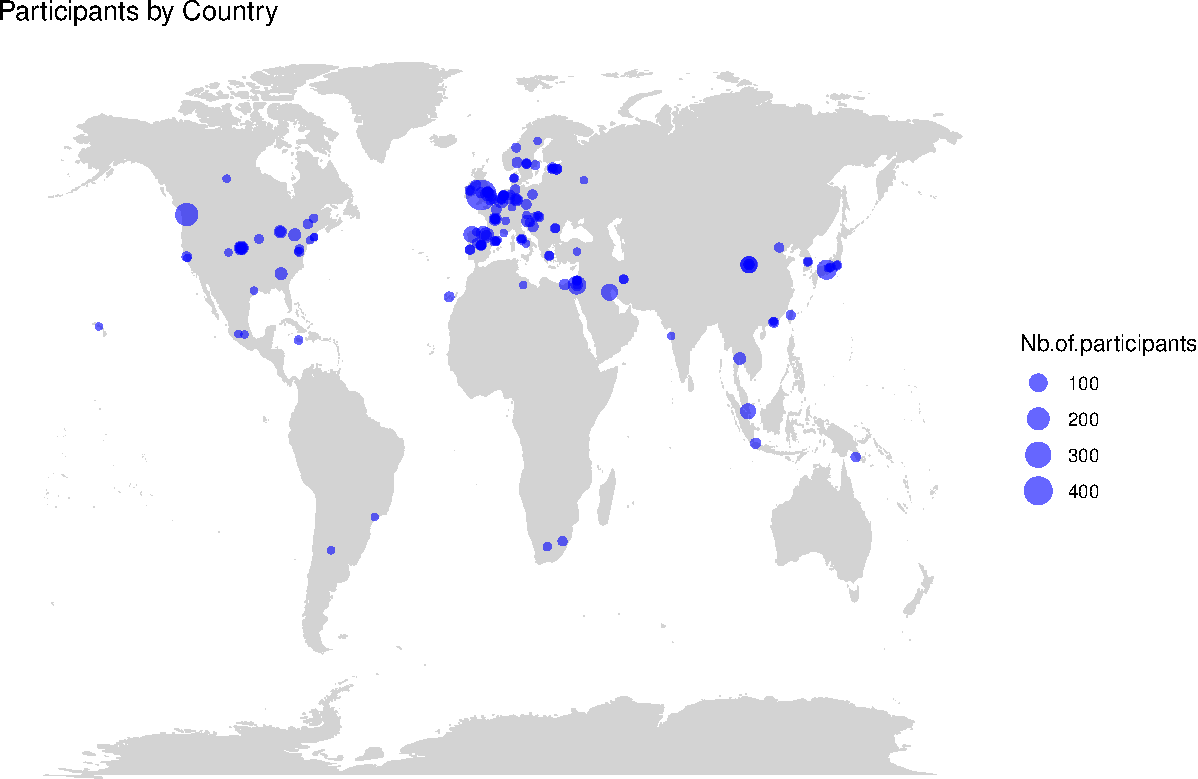
\includegraphics{CHILDES_short_files/figure-latex/unnamed-chunk-1-1.pdf}
\caption{\label{fig:unnamed-chunk-1}World map showing corpus. Size proportional to number of children per corpus}
\end{figure}

We assessed the extent to which the countries with data in our sub-sample of CHILDES were a representative sample of countries in the world. Density plots are portrayed in Figure 2.

By comparing our sub-sample of CHILDES to the world statistics using unpaired samples t-tests without assuming equality of variance (Welch's t). Countries in our sub-sample of CHILDES had a higher proportion of the population completing lower secondary school than the world wide sample (\% compl. LSS, t(130.41)=-6.19, p = 0); they were more urban (\% urban, t(79.48)=-3.44, p = 0); richer (log GDP per capita, t(102.35)=-6.02, p = 0) and had smaller households (average household size, t(118.80)=7.12, p = 0) and less average number of members under the age of 15 (average under 15 size, t(26.12)=5.01, p = 0).

\subsection{Corpus-level}\label{corpus-level}

We then investigated at the corpus level the variables described in Table 2. The information collected allows us to have more detail about the characteristics of the individual families that compose our sub-sample of CHILDES. However, it is important to acknowledge that for the majority of the corpora, this information was missing, not known, or not provided.

\subsubsection{SES}\label{ses}

Of the 102 (43\%) corpora, 5 were described as having low SES; 16 were described as spanning both lower and middle or higher SES; and 81 were described as middle or higher SES exclusively (79\%). Given that most countries represented in our sub-sample of CHILDES are in the OECD, we can compare this proportion with the proportion of the population in these countries that are middle class. According to a 2016 report, ``Almost two-thirds of people live in middle-income households in OECD countries'', for whom ``household net income {[}is{]} between 0.75 and 2 times the median''. Thus, middle and higher-class participants appear to be over-represented in our sub-sample of CHILDES data.

For socioeconomic status, there were 106 missing values (33\%). Of the remaining 215 samples, were described as having low SES; were described as spanning both lower and middle or higher SES; and were described as middle or higher SES exclusively. Given that most countries represented in CHILDES are in the Organization for Economic Cooperation and Development (OECD, 0 out of the 321 corpora), we can compare this proportion with the proportion of the population in these countries that are middle class. According to a 2016 report, ``Almost two-thirds of people live in middle-income households in OECD countries'', for whom ``household net income {[}is{]} between 0.75 and 2 times the median''. Thus, middle and higher class participants appear to be over-represented in CHILDES data, composing 81\% of available data.

\paragraph{Education}\label{education}

76\% of the corpora (n = 58) include children whose parents had at least a graduate, if not a postgraduate, degree. 4\% (n=3 ) had at least some parents with primary-level education; 12\% (n=9) had parents with secondary school education as the lower bound of the education range, and a further 8\% (n=6) had some college as the lower bound. 4 corpora were described as ``diverse'', without clarifying the range of education covered. These numbers do not accurately represent the demographics of the countries they were obtained from. For instance, while the U.S. Census Bureau reported that only 36\% of the adult population held a bachelor's degree or higher in 2020, our data indicates that 100\% of the corpora of the parents from the United States had a college education or higher. As seen in Figure 3, the same result is seen for corpus from China, Denmark, Egypt, Hong Kong, Hungary, Israel, Italy, Japan, Mexico, The Netherlands, Poland, Russia, Singapore, South Korea, Switzerland and the United States where 100\% of parents with data are college-educated or above. Thus, it seems that our sub-samples of CHILDES are very skewed toward higher-educated parents.

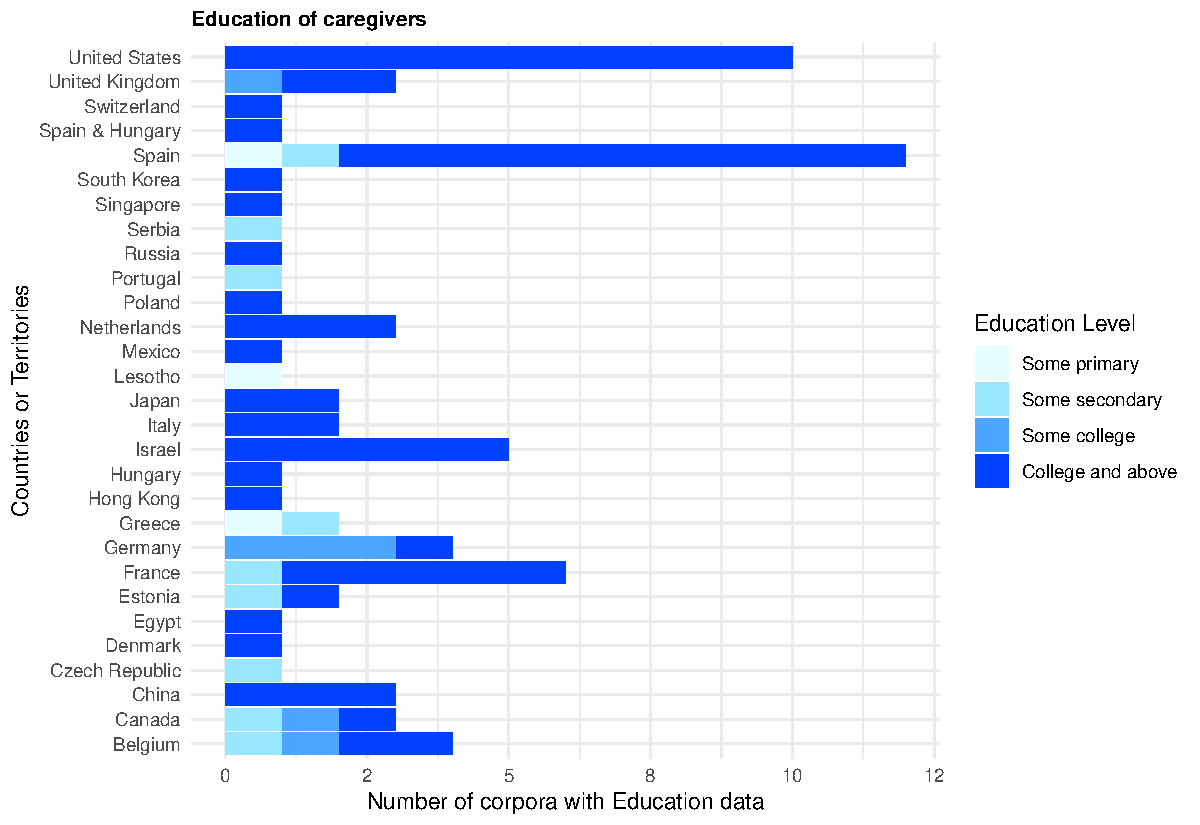
\includegraphics{CHILDES_short_files/figure-latex/figure3 -1.pdf}
\#\#\#\# Occupation
Professions were overall varied. The majority, comprising62\% (n=52), was associated with the field of education. Notably, within this category, 56\% (n=47) of the individuals were identified as parents with professions linked to graduate-level education. This included roles such as Master's or Ph.D.~students, professors, linguists, researchers, scientists, and academics. Some of the other occupations reported were psychologists, speech therapist or home makers.

\subsubsection{Urbanization}\label{urbanization-1}

78\% of the corpora (n=51) corpora were described as industrialized or urban, and an additional one as both rural and urban. Only 7 corpora were described as farming or rural. In these same countries, the proportion of the population residing in urban settings was 76\%, suggesting that samples were not representative of their countries in terms of rural versus urban settings either.

\begin{figure}
\centering
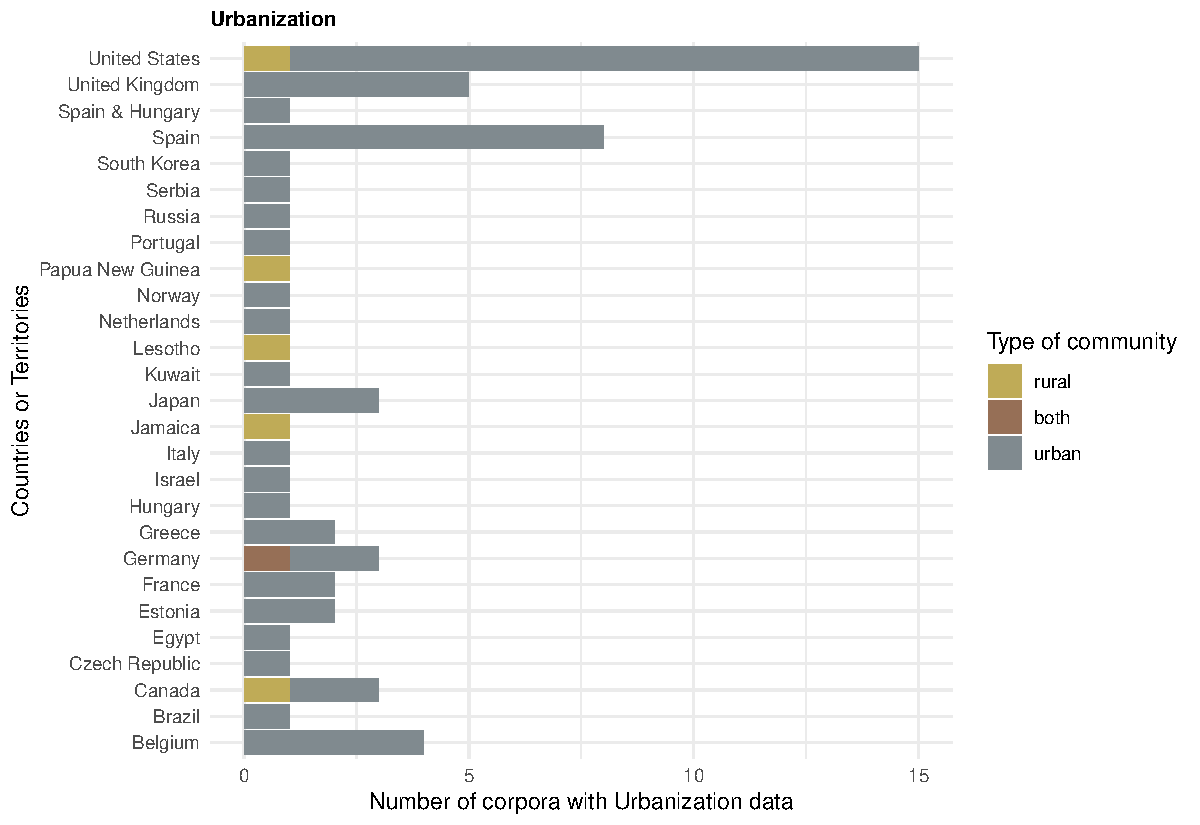
\includegraphics{CHILDES_short_files/figure-latex/figure4-1.pdf}
\caption{\label{fig:figure4}Urbanization by country.}
\end{figure}

\subsubsection{Family structure}\label{family-structure-1}

\paragraph{Nuclear households}\label{nuclear-households}

As for household composition, 60 corpora (87\%) were based on nuclear families; 7 extended families(10\%); and in 2 corpora the structure was varied (3\%). We compare side by side the average per country of the nuclear households (the sum of the percentages of couples with children households, and single parents with children households; United Nations, 2022).

\paragraph{Sibling presence}\label{sibling-presence}

A majority of corpora in our sub-sample of CHILDES include children who have siblings. In fact, only 28\% of corpora (among the 93 corpora having information on siblings) were constituted exclusively of children with no siblings, and the remaining had at least one sibling, with the overall average being 0.8 siblings. Since 83\% of countries in CHILDES are in the OECD, we draw a comparison point for such countries: 46\% of children had no siblings in OECD countries according to 2015 data. In this sense, children with no siblings appear to be under-represented in CHILDES.

\subsubsection{Languages}\label{languages}

We had two variables of interest here: language spoken in the corpus and lingual status. A total of 62 different languages or language combinations (for bilingual and multilingual children) were reportedly spoken in the corpora.

\begin{center}
\begin{ThreePartTable}

\begin{longtable}{lccc}\noalign{\getlongtablewidth\global\LTcapwidth=\longtablewidth}
\caption{\label{tab:tab4}Total number of participants per language,}\\
\toprule
Monolingual\_Language & \multicolumn{1}{c}{Total\_Participants} & \multicolumn{1}{c}{Multilingual\_Languages} & \multicolumn{1}{c}{Total\_Participants\_Multilingual}\\
\midrule
\endfirsthead
\caption*{\normalfont{Table \ref{tab:tab4} continued}}\\
\toprule
Monolingual\_Language & \multicolumn{1}{c}{Total\_Participants} & \multicolumn{1}{c}{Multilingual\_Languages} & \multicolumn{1}{c}{Total\_Participants\_Multilingual}\\
\midrule
\endhead
Afrikaans & 2.00 & Dutch/English, Dutch/French & 35.00\\
Arabic (Egyptian or Kuwaiti) & 80.00 & Dutch/Italian & 4.00\\
Basque & 46.00 & Spanish/Catalan & 6.00\\
Cantonese & 8.00 & Spanish/Galician & 66.00\\
Catalan & 17.00 & English/Cantonese & 9.00\\
Cree & 1.00 & English/French & 12.00\\
Croatian & 3.00 & English/Hebrew & 1.00\\
Czech & 6.00 & English/Japanese & 1.00\\
Danish & 2.00 & English/Japanese/Danish & 1.00\\
Dutch & 23.00 & English/Mandarin & 55.00\\
English & 210.00 & English/Mandarin/Cantonese & 11.00\\
Estonian & 32.00 & English/Russian & 22.00\\
Farsi & 5.00 & English/Spanish & 12.00\\
French & 46.00 & French/Russian & 1.00\\
German & 46.00 & Hungarian/Catalan/Spanish & 1.00\\
Greek & 6.00 & Hungarian/Farsi/English & 2.00\\
Hebrew & 122.00 & German/Spanish & 9.00\\
Hungarian & 8.00 & Italian/Japanese & 1.00\\
Icelandic & 1.00 & Italian/German & 2.00\\
Indonesian & 8.00 & Portuguese/Swedish/English & 3.00\\
Irish & 7.00 & NA & NA\\
Italian & 8.00 & NA & NA\\
Jamaican & 2.00 & NA & NA\\
Japanese & 148.00 & NA & NA\\
Korean & 4.00 & NA & NA\\
Mandarin & 157.00 & NA & NA\\
Norwegian & 11.00 & NA & NA\\
Nungon & 5.00 & NA & NA\\
Polish & 4.00 & NA & NA\\
Portuguese (Brazilian or European) & 9.00 & NA & NA\\
Romanian & 6.00 & NA & NA\\
Russian & 2.00 & NA & NA\\
Serbian & 8.00 & NA & NA\\
Sesotho & 4.00 & NA & NA\\
Slovenian & 20.00 & NA & NA\\
Spanish & 75.00 & NA & NA\\
Swedish & 9.00 & NA & NA\\
Taiwanese & 4.00 & NA & NA\\
Tamil & 1.00 & NA & NA\\
Thai & 18.00 & NA & NA\\
Turkish & 1.00 & NA & NA\\
Welsh & 475.00 & NA & NA\\
\bottomrule
\end{longtable}

\end{ThreePartTable}
\end{center}

About a third (32\%) of the included corpora that had available data for this variable (N = 110) were not monolingual. It is hard to find reliable estimates of the percentage of the population which is not monolingual in the world or in the countries represented in our sub-sample of CHILDES, but for instance, in Europe in 2016, 65\% of adults reported knowing multiple languages (Eurostat, 2022). According to such estimates, even if samples are linguistically diverse, it would appear that input data in our sub-sample of CHILDES under-represents bilingual and multilingual households.

\section{Discussion}\label{discussion}

\newpage

\section{References}\label{references}


\end{document}
